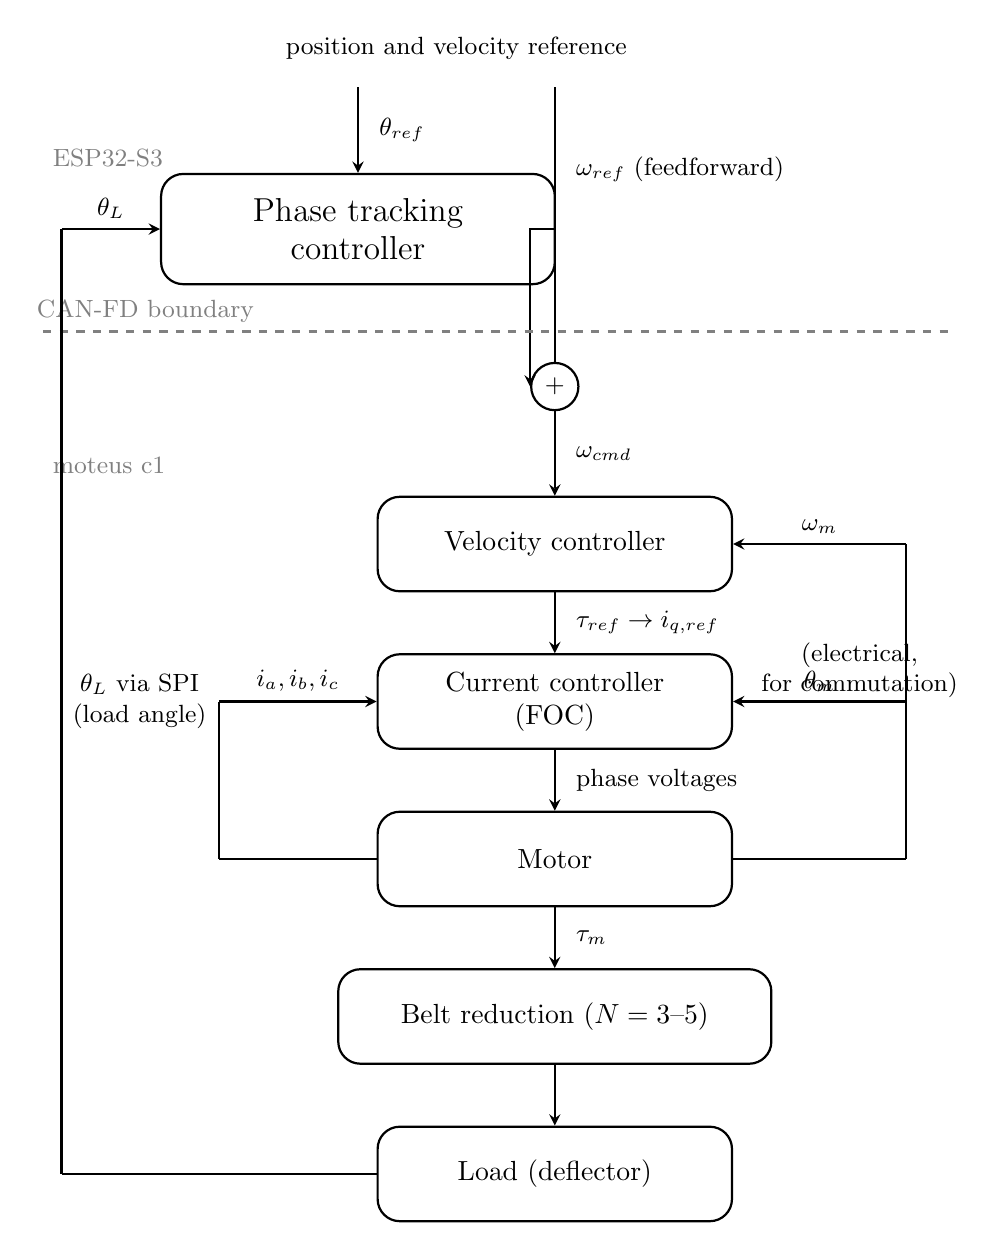
\begin{tikzpicture}[
		box/.style={
				draw, rounded corners=8pt, thick,
				minimum width=5cm, minimum height=1.4cm,
				align=center, font=\large
			},
		smallbox/.style={
				draw, rounded corners=8pt, thick,
				minimum width=4.5cm, minimum height=1.2cm,
				align=center, font=\normalsize
			},
		container/.style={
				draw, rounded corners=10pt, thick, dashed,
				inner sep=10pt
			},
		sum/.style={
				draw, circle, thick, inner sep=1pt,
				minimum size=6mm, font=\small
			},
		arr/.style={->, >=stealth, thick},
		line/.style={thick},
		lbl/.style={font=\small, align=center},
		boundary/.style={dashed, thick, gray}
	]

	% Phase tracking controller
	\node[box] (ptc) at (0, 0) {Phase tracking\\controller};

	% Summing junction
	\node[sum] (sum) at (2.5, -2.0) {$+$};

	% Velocity controller
	\node[smallbox] (vel) at (2.5, -4.0) {Velocity controller};

	% Current controller
	\node[smallbox] (cur) at (2.5, -6.0) {Current controller\\(FOC)};

	% Motor
	\node[smallbox] (motor) at (2.5, -8.0) {Motor};

	% Belt reduction
	\node[smallbox, minimum width=5.5cm] (belt) at (2.5, -10.0) {Belt reduction ($N=3\text{–}5$)};

	% Load
	\node[smallbox] (load) at (2.5, -12.0) {Load (deflector)};

	% Reference inputs (top)
	\coordinate (refin)  at (0,  1.8);
	\coordinate (ffin)   at (2.5, 1.8);

	\draw[arr] (refin) -- node[lbl, right=4pt, pos=0.5] {$\theta_\text{ref}$} (ptc.north);
	\draw[line] (ffin) -- node[lbl, right=4pt, pos=0.3] {$\omega_\text{ref}$ (feedforward)} (sum.north);

	% Common input label above
	\node[lbl] at (1.25, 2.3) {position and velocity reference};

	% PTC -> sum
	\draw[arr] (ptc.east) -| (sum.west);

	% sum -> velocity controller
	\draw[arr] (sum.south) -- node[lbl, right=4pt] {$\omega_\text{cmd}$} (vel.north);

	% velocity -> current
	\draw[arr] (vel.south) -- node[lbl, right=4pt] {$\tau_\text{ref} \to i_{q,\text{ref}}$} (cur.north);

	% current -> motor
	\draw[arr] (cur.south) -- node[lbl, right=4pt] {phase voltages} (motor.north);

	% motor -> belt
	\draw[arr] (motor.south) -- node[lbl, right=4pt] {$\tau_m$} (belt.north);

	% belt -> load
	\draw[arr] (belt.south) -- (load.north);

	% CAN-FD boundary line
	\draw[boundary] (-4.0, -1.3) -- (7.5, -1.3);
	\node[lbl, gray] at (-2.7, -1.05) {CAN-FD boundary};

	% ESP32 label
	\node[lbl, gray, anchor=west] at (-4.0, 0.9) {ESP32-S3};

	% moteus label
	\node[lbl, gray, anchor=west] at (-4.0, -3.0) {moteus c1};

	% Feedback: motor -> velocity controller (omega_m)
	\draw[line] (motor.east) -- ++(2.2, 0) coordinate (fb1);
	\draw[line] (fb1) -- (fb1 |- vel.east);
	\draw[arr]  (fb1 |- vel.east) -- node[lbl, above, pos=0.5] {$\omega_m$} (vel.east);

	% Feedback: motor -> current controller (theta_m for commutation)
	\draw[line] (motor.east) ++(2.2, 0) -- ++(0, 2.0) coordinate (fb2);
	\draw[line] (fb2) -- (fb2 |- cur.east);
	\draw[arr]  (fb2 |- cur.east) -- node[lbl, above, pos=0.5] {$\theta_m$} (cur.east);
	\node[lbl, anchor=west] at (5.0, -5.6) {(electrical,\\for commutation)};

	% Feedback: phase currents -> current controller
	\draw[line] (motor.west) -- ++(-2.0, 0) coordinate (fbc);
	\draw[line] (fbc) -- (fbc |- cur.west);
	\draw[arr]  (fbc |- cur.west) -- node[lbl, above, pos=0.5] {$i_a, i_b, i_c$} (cur.west);

	% Feedback: load -> phase tracking controller (theta_L)
	\draw[line] (load.west) -- ++(-4.0, 0) coordinate (fbl);
	\draw[line] (fbl) -- (fbl |- ptc.west);
	\draw[arr]  (fbl |- ptc.west) -- node[lbl, above, pos=0.5] {$\theta_L$} (ptc.west);
	\node[lbl, anchor=east] at (-1.8, -6.0) {$\theta_L$ via SPI\\(load angle)};

\end{tikzpicture}
